\documentclass[sigconf,review]{acmart}



%% Copyright information
\setcopyright{acmcopyright} % TODO: copyright?
\copyrightyear{2022}
\acmYear{2022}
\acmDOI{10.1145/1122445.1122456} % TODO: DOI?

%% These commands are for a PROCEEDINGS abstract or paper.
\acmConference[Pittsburgh '22]{Pittsburgh '22: NIER - New Ideas and Emerging
Results (ICSE 2022)}{May 21--29, 2022}{Pittsburgh, PA, USA}
\acmBooktitle{Pittsburgh '22: NIER - New Ideas and Emerging Results (ICSE 2022),
May 21--29, 2022, Pittsburgh, PA, USA} \acmISBN{978-1-4503-XXXX-X/18/06}
% TODO: ISBN

%% Packages

% \usepackage[paperwidth=8.50in, paperheight=11in]{geometry} %% option clash
\usepackage[T1]{fontenc}
%\usepackage[latin1]{inputenc}

% \usepackage[protrusion=true,expansion=true]{microtype} %% option clash

% for inline lists
\usepackage[inline]{enumitem}
% for nice internal links
\usepackage{hyperref}

\begin{document}

\title{A Sustainable Approach to Developing Software in Well Understood Domains}

\author{Jacques Carette}
\orcid{0000-0001-8993-9804}
\affiliation{
  \department{Computing and Software}
  \streetaddress{1280 Main Street West}
  \institution{McMaster University}
  \city{Hamilton}
  \state{Ontario}
  \postcode{L8S 4L8}
  \country{Canada}}
\email{carette@mcmaster.ca}

\author{Spencer Smith}
\orcid{0000-0002-0760-0987}
\affiliation{
  \department{Computing and Software}
  \streetaddress{1280 Main Street West}
  \institution{McMaster University}
  \city{Hamilton}
  \state{Ontario}
  \postcode{L8S 4L8}
  \country{Canada}}
\email{smiths@mcmaster.ca}

\author{Jason Balaci}
%\orcid{0000-0002-0760-0987}
\affiliation{
  \department{Computing and Software}
  \streetaddress{1280 Main Street West}
  \institution{McMaster University}
  \city{Hamilton}
  \state{Ontario}
  \postcode{L8S 4L8}
  \country{Canada}}
\email{balacij@mcmaster.ca}

\begin{abstract}
  Current software development methods are too general to be ideally suited to
  sustainable development of software in well understood domains.  A software
  domain is considered well understood if the domain knowledge can be codified,
  the computational interpretation of the domain knowledge is clear and the
  engineering of code to perform the computations is well understood.  When the
  domain is well-understood developers can invest in building an infrastructure
  that will facilitate long-lived software.  In this paper we present an
  idealized process that codifies domain knowledge and employs generative
  techniques to create the required software artifacts.  The methodology is
  illustrated via an example of software used to predict the risk of breakage
  for glass windows subjected to a nearby explosion.
\end{abstract}


% Generator:   http://dl.acm.org/ccs.cfm
% TODO: This is a temporary CCSXML and \ccsdesc list
\begin{CCSXML}
<ccs2012>
   <concept>
       <concept_id>10011007.10011006.10011066.10011070</concept_id>
       <concept_desc>Software and its engineering~Application specific development environments</concept_desc>
       <concept_significance>300</concept_significance>
       </concept>
   <concept>
       <concept_id>10011007.10011074.10011075.10011076</concept_id>
       <concept_desc>Software and its engineering~Requirements analysis</concept_desc>
       <concept_significance>300</concept_significance>
       </concept>
   <concept>
       <concept_id>10011007.10011006.10011060.10011690</concept_id>
       <concept_desc>Software and its engineering~Specification languages</concept_desc>
       <concept_significance>300</concept_significance>
       </concept>
   <concept>
       <concept_id>10011007.10011074.10011092.10011782</concept_id>
       <concept_desc>Software and its engineering~Automatic programming</concept_desc>
       <concept_significance>500</concept_significance>
       </concept>
 </ccs2012>
\end{CCSXML}

\ccsdesc[300]{Software and its engineering~Application specific development environments}
\ccsdesc[300]{Software and its engineering~Requirements analysis}
\ccsdesc[300]{Software and its engineering~Specification languages}
\ccsdesc[500]{Software and its engineering~Automatic programming}
%% End of generated code

\keywords{code generation, document generation, knowledge capture,
  software engineering, scientific software}

% set up math environment
\newtheorem{defn}{Definition}

\maketitle

\section{What is ``well understood'' Software?}\label{ch:wellUnderstood}

\begin{defn}
A software domain is \emph{well understood} if
\begin{enumerate}
\item the Domain Knowledge (DK) is codified,
\item the computational interpretation of the DK is clear,
\item the engineering of code to perform said computations is well
understood.
\end{enumerate}
\end{defn}

By \emph{codified}, we mean that the knowledge exists in standard form in a
variety of textbooks. For example, many domains of knowledge in engineering use
standard differential equations as models. Furthermore, the quantities of
interest are known, given standard names and standard units. In other words,
standard vocabulary has been established over time and the body of knowledge is
uncontroversial.

We can further refine these high level ideas as follows, where we use
the same numbering as above to indicate which part of the definition is
being directly refined, but where the refinement nevertheless should be
understood more holistically.
\begin{enumerate}
\item Models in the DK \emph{can be} written formally.
\item Models in the DK \emph{can be} turned into functional relations by
 existing mathematical steps.
\item Turning these functional relations into code is an understood
 transformation.
\end{enumerate}
Perhaps the most important aspect of this refinement is that the last two parts
deeply involve \emph{choices}: What quantities are considered inputs, outputs
and parameters to make the model functional? What programming language?  What
software architecture data-structures, algorithms, etc.?

\emph{Well understood} does not imply \emph{choice free}.  For instance,
different authors would make different choices when writing a small script to
move files.  Depending on the author's style, this can be easily written as a
Shell script, or in Python or in Haskell. In all cases, assuming the author
chooses a language in which they are fluent, the job will be entirely
straightforward because the domain is well understood.

Code is \emph{not} the only artifact that matters.  Our definition for well
understood also applies, equally importantly, to documentation for humans, as
follows:
\begin{enumerate}
\item The meaning of the models is understood at a human-pedagogical
level, i.e. it is explainable.
\item Combining models is also explainable. Thus \emph{transformers}
  %we mentioned before %this is actually the first time transformers are mentioned
  simultaneously operate on mathematical representations
and on explanations. This requires that English descriptions also be
captured in the same manner as the formal-mathematical knowledge.
\item Similarly, the \emph{transformers} that arise from making software
oriented decisions should be captured with a similar mechanism, and also include
English explanations.
\end{enumerate}

We dub these \emph{triform theories}, as a nod to \emph{biform
theories}~\cite{Farmer2007}. The idea is that we couple 
\begin{enumerate*}
\item an axiomatic description,
\item a computational description, and
\item an English description
\end{enumerate*}
of a concept.

Different kinds of choices are embedded in the different kinds of knowledge.
They can show up simply as \emph{parameters}, for example the acceleration due
to gravity constant associated with a planet. They can also shows up as
different transformers, for example turning $F - m\cdot a = 0$ into $F\left(m,
a\right) = m\cdot a$, i.e. from a conservation law into a computation. Note
that, for motion computation, that same conservation law is often rewritten as
$a\left(m,F\right) = F/m$ as part of solving $a = \ddot{x}$ to obtain a position
($x$) as a function of time ($t$). We also get choices of phrasing, which are
equivalent but may be more adequate in a given context.

\section{Ideal Process}\label{ch:process}

When a domain is well understood, codifying the domain knowledge is an option.
However, codification requires significant effort; this effort is only
worthwhile when the goal is long-lived software.  Moreover, the process that is
followed needs to explicitly take advantage of the well understood domain
knowledge.  So what would be a reasonable process for building a piece of
software, assuming some kind of infrastructure exists for recording the kind of
knowledge outlined in~\autoref{ch:wellUnderstood}?  Below we outline a
chronological ``story'' of such an idealized process.  We are \textbf{not}
outlining the actual process to follow, but rather the \emph{idealized process}
(influenced by Parnas's paper on faking a rational design process
\cite{Parnas1986}).

\begin{enumerate}
\item\label{it:problem} Have a problem to solve, or task to achieve, which
falls into the realm where \emph{software} is likely to be the central part of
the solution.
\item\label{it:understood} Convince oneself that the underlying problem domain
is \emph{well understood}, as defined in~\autoref{ch:wellUnderstood}.
\item\label{it:probdesc} Describe the problem:
  \begin{enumerate}
  \item Find the base knowledge (theory) in the pre-existing library
    or, failing that, write it if it does not yet exist,
  \item Assemble the ingredients into a coherent narrative,
  \item Describe the characteristics of a good solution,
  \item Come up with basic examples (to test correctness, intuitions, etc).
  \item Identify the naturally occurring known quantities associated to the
    problem domain, as well as some desired quantities. For example,
    some problems naturally involve lengths lying in particular
    ranges, while others will involve reagent concentrations, again
    in particular ranges.
  \end{enumerate}
\item\label{it:refine} Describe, by successive transformations, how the natural
knowledge can be turned from a set of relations (and constraints) into a
deterministic\footnote{For the moment, we explicitly restrict our domain to
deterministic solutions, as a meta-design choice. This can be expanded later.}
input-output process.
  \begin{enumerate}
  \item This set of relations might require \emph{specializing} the
    theory (eg. from $n$-dimensional to $2$-dimensional, assuming no
    friction, etc).  These \emph{choices} need to be documented, and are
    a crucial aspect of the solution process. The \emph{rationale} for the
    choices should also be documented. Lastly, whether these choices are
    likely or unlikely to change in the future should be recorded.
  \item This set of choices is likely dependent, and thus somewhat ordered.
  In other words, some \emph{decisions} will enable other choices to be
  made that would otherwise be unavailable. Eg: some data involved in the
  solution process is orderable, so that sorting is now a possibility that
  may be useful.
  \end{enumerate}
\item\label{it:tocode} Describe how the computation process from step
\ref{it:refine} can be turned into code. Note that the same kinds of choice
can occur here.
\item\label{it:recipe} Turn the steps (i.e.\ from items~\ref{it:refine} and
\ref{it:tocode}) into a \emph{recipe}, aka program, that weaves together all the
information into a variety of artifacts (documentation, code, build scripts,
test cases, etc). These can be read, or executed, or \ldots\, as appropriate.
\end{enumerate}

While this last step might appear somewhat magical, it isn't. The whole point of
defining \emph{well understood} is to enable that last step. A suitable
knowledge encoding is needed to enable it, but this step is a reflection of what
humans currently themselves do when assembling their software and associated
artifacts. We are merely being explicit about how to go about mechanizing these
steps.

What is missing is an explicit \emph{information architecture} of each of
the necessary artifact. In other words, what information is necessary to
enable the mechanized generation of each artifact? It turns out that many
of them are quite straightforward.

It is worthwhile to note that way too many research projects skip
step~\ref{it:problem} and~\ref{it:probdesc}: in other words, they never really
write down what problem they're trying to solve. This is part of the
\textbf{tacit knowledge} of a lot of research software.  It is crucial to our
whole process that this knowledge go from tacit to explicit. This is also one
of the fundamental recognitions of \emph{Knowledge
Management}~\cite{KM-textbook}.

% TODO: insert graphical illustration of the funnel from information to
% softifacts.

\section{Example}\label{ch:example}

Implementation found in Drasil~\cite{}.

\begin{figure*}[h]
  \centering
  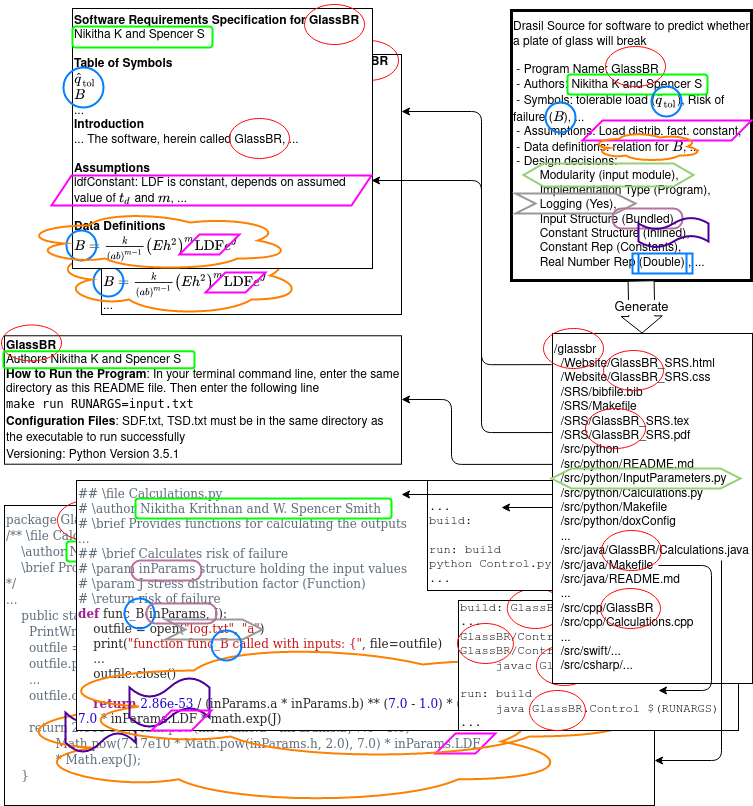
\includegraphics[width=\linewidth]{assets/DrasilSupportsChange-right-portrait-overlapped-ungrouped-v1.drawio.png}
  \caption{TODO: caption}
  \Description{TODO: description}
\end{figure*}

\section{Concluding Remarks} \label{ch:concluding_remarks}

Concluding remarks.

%% Bibliography
\bibliographystyle{ACM-Reference-Format}
\bibliography{References}

\end{document}

% Good quotes:
% \begin{itemize}
% \item metaprograms are just programs
% \item models outside an integrated toolchain are insufficiently useful
% \end{itemize}
